\subsection{Визначення бізнес-вимог}
\subsubsection{Опис предметної області}

Суб'єкти:

\begin{itemize}
\item Слухачі --- особи, що можуть записуватися на курси або вже записані на деякі курси.
\item Викладачі --- особи, що ведуть певні курси.
\item Оператори --- допоміжний персонал та довірені особи, що займаються записом слухачів, приймають оплати та формують звіти.
\item Адміністратори --- особи, що безпосередньо завідують курсами, дають завдання операторам та можуть виконувати їх функції.
\end{itemize}

\noindent
\begin{tikzpicture}
\makeatletter
\tikzset{
 circle connection bar/.style={rectangle,draw=\tikz@concept@color,every circle connection bar},
 every concept/.append style={minimum size=0cm, color=black, fill=white},
 concept/.style={circle,draw=\tikz@concept@color,every concept},
 every node/.append style={concept}
} \makeatother
\path[
 mindmap,
 scale=0.8,
 level 1 concept/.append style={sibling angle=120},
 level 2 concept/.append style={sibling angle=60},
 level 3 concept/.append style={sibling angle=30},
 level 4 concept/.append style={sibling angle=32,text width=1cm},
 sys/.style={concept, font=\footnotesize},
]
node [sys] {Система обліку платних курсів\\із підтримкою самостійного запису слухачів через мережу Інтернет} [clockwise from=210]
 child {
  node {Вхідний потік} [clockwise from=330]
   child { node {Хто?} [clockwise from=340]
    child { node {Оператори} }
    child { node [text width=1.4cm] {Адміністратор} }
    child [sibling angle=32] { node {Слухачі} [clockwise from=330]
     child { node {Студенти} }
     child { node {Сторонні} }
    }
   }
   child { node {Що?} [clockwise from=320]
    child { node {Дані слухачів} }
    child { node {Курси} }
    child { node {Дані викладачів} }
    child { node [text width=1.2cm] {Коефіціенти} }
    child { node {Розклад курсів} }
   }
   child { node {Де?} [clockwise from=200]
    child { node {Web-сайт} }
    child { node {Кафедра СПЗ} }
   }
   child { node {Коли?}  [clockwise from=180]
    child { node {Початок чверті} }
    child { node {Довільно} }
   }
   child { node {Як?} [clockwise from=150]
    child { node {Ручне введення} }
    child [sibling angle=45] { node {Імпорт з системи електронного деканату} }
   }
 } child {
  node [text width=2.5cm]{Внутрішній потік} [clockwise from=210]
   child { node {Хто?} }
   child { node {Що?} 
    child { node [text width=1.2cm] {Збереження даних} }
    child { node {Контроль цілісності} }
    child { node [text width=1.2cm] {Розрахунок вартості курсу} }
   }
   child { node {Де?} [clockwise from=105]
    child { node {Web-сервер} }
    child { node {СКБД} }
   }
   child { node {Коли?} [clockwise from=60]
    child { node {Постійно} }
   }
   child { node {Як?} [clockwise from=30]
    child { node {Формула} }
   }
 } child {
  node {Вихідний потік} [clockwise from=90]
   child { node {Хто?} [clockwise from=120]
    child { node {Викладачі} }
    child { node {Оператори} }
    child { node [text width=1.4cm] {Адміністратор} }
    child { node {Слухачі} [clockwise from=30]
     child { node {Студенти} }
     child { node {Сторонні} }
    }
   }
   child { node {Що?} [clockwise from=35]
    child { node [text width=1.2cm] {Сповіщення} }
    child { node {Звіти} 
     child { node {За період} }
     child { node {За курсом} }
    }
    child { node {Розклад} }
   }
   child { node {Де?} [clockwise from=10]
    child { node {Web-сайт} }
    child { node {Кафедра СПЗ} }
    child { node [text width=1.2cm] {Бухгалтерія} }
   }
   child { node {Коли?} [clockwise from=340]
    child { node {Кінець семестру} }
    child { node {Під час курсів} }
   }
   child { node {Як?} [clockwise from=300]
    child { node {Звіти} [clockwise from=320]
     child { node {У файл} }
     child { node {Друк} }
    }
    child { node [text width=1.2cm] {Сповіщення} [clockwise from=280]
     child { node {На e-mail} }
     child [sibling angle=40] { node {На сайті} }
    }
   }
 };
\end{tikzpicture}
\imglabel{Мозкова карта}

\subsubsection{Назва продукту}

<<К\&П 2014>> --- скорочення від <<Курси та платежі>>, 2014 --- рік розробки базової версії продукту.

\subsubsection{Проблеми}

\begin{enumerate}
 \item Відсутність актуальної інформації про наявні курси в мережі Інтернет.
 \item Необхідність слухачам відвідувати кафедру СПЗ для реєстрації на курс, черги, ручне введення контактних даних через операторів.
 \item Зберігання відомостей про курси у текстових документах та ручне формування звітів.
 \item Ручне заповнення бланку договору.
 \item Слухачі забувають розклад курсів, а викладачі шукають вільну аудиторію для проведення курсів.
\end{enumerate}

\nopagebreak[4]
\subsubsection{Аналогічні системи}

\newcommand{\ltwoc}[1]{\multicolumn{2}{l|}{\parbox[t]{4cm}{#1}}}
\newcommand{\rtwoc}[1]{\multicolumn{2}{l|}{\parbox[t]{5cm}{#1}}}
\setlength{\tabcolsep}{0.4pt}
\begin{tabular}{|p{3.5cm}|p{2cm}|p{2cm}|p{2.8cm}|p{2.2cm}|p{3.5cm}|}
 \hline
 \backslashbox[3.5cm]{Назва}{Проблема} & \Centering 1 & \Centering 2 & \Centering 3 & \Centering 4 & \Centering 5 \\\hline
 1C: Бухгалтерія & \ltwoc{Зовнішній сайт +\\web-сервіс} & Бібліотека стандартних підсистем + бібліотека електронних документів & Бібліотека електронних документів & Зовнішня розсилка сповіщень + web-сервіс \\\hline
 Парус & \ltwoc{Зовнішній сайт +\\сервіс реплікації} & \rtwoc{Конструктор галузевих рішень + сервіс звітності} & Зовнішня розсилка сповішень + сервіс реплікації \\\hline
 1C-Бітрікс: Внутрішній портал навчального закладу & \ltwoc{Групи за предметами} & --- & --- & Жива стрічка, календар \\\hline
 Moodle & Створен\-ня та пошук курсів & Само\-стійна реєстрація на курси & --- & --- & Календар \\\hline
 Веб-застосунок MS Access + SharePoint & Предс\-тавлення списку & Форми & \rtwoc{Шаблонні звіти або інтеграція з MS Access для робочого столу для формування складних звітів} & Представлення таблиць, розсилка сповіщень за допомогою макросів MS Access для робочого столу \\\hline
\end{tabular}

\subsubsection{Цілі}

\begin{itemize}
 \item Зменшення часу реєстрації на курс
 \item Зменшення часу формування звітів з даних про курси
 \item Зменшення часу укладення договору
 \item Зменшення часу отримання інформації про наявні курси, розклад курсів та вільні аудиторії
\end{itemize}

\newpage

\subsection{Визначення власних вимог}

\subsubsection{Діаграма варіантів використання}

\begin{flushright}
 \begin{textblock*}{5cm}(12cm,5cm)
  \footnotesize Умовні позначення:
   \begin{itemize}
    \item C --- створення
    \item R --- перегляд
    \item U --- редагування
    \item D --- видалення
   \end{itemize}
 \end{textblock*}
\end{flushright}

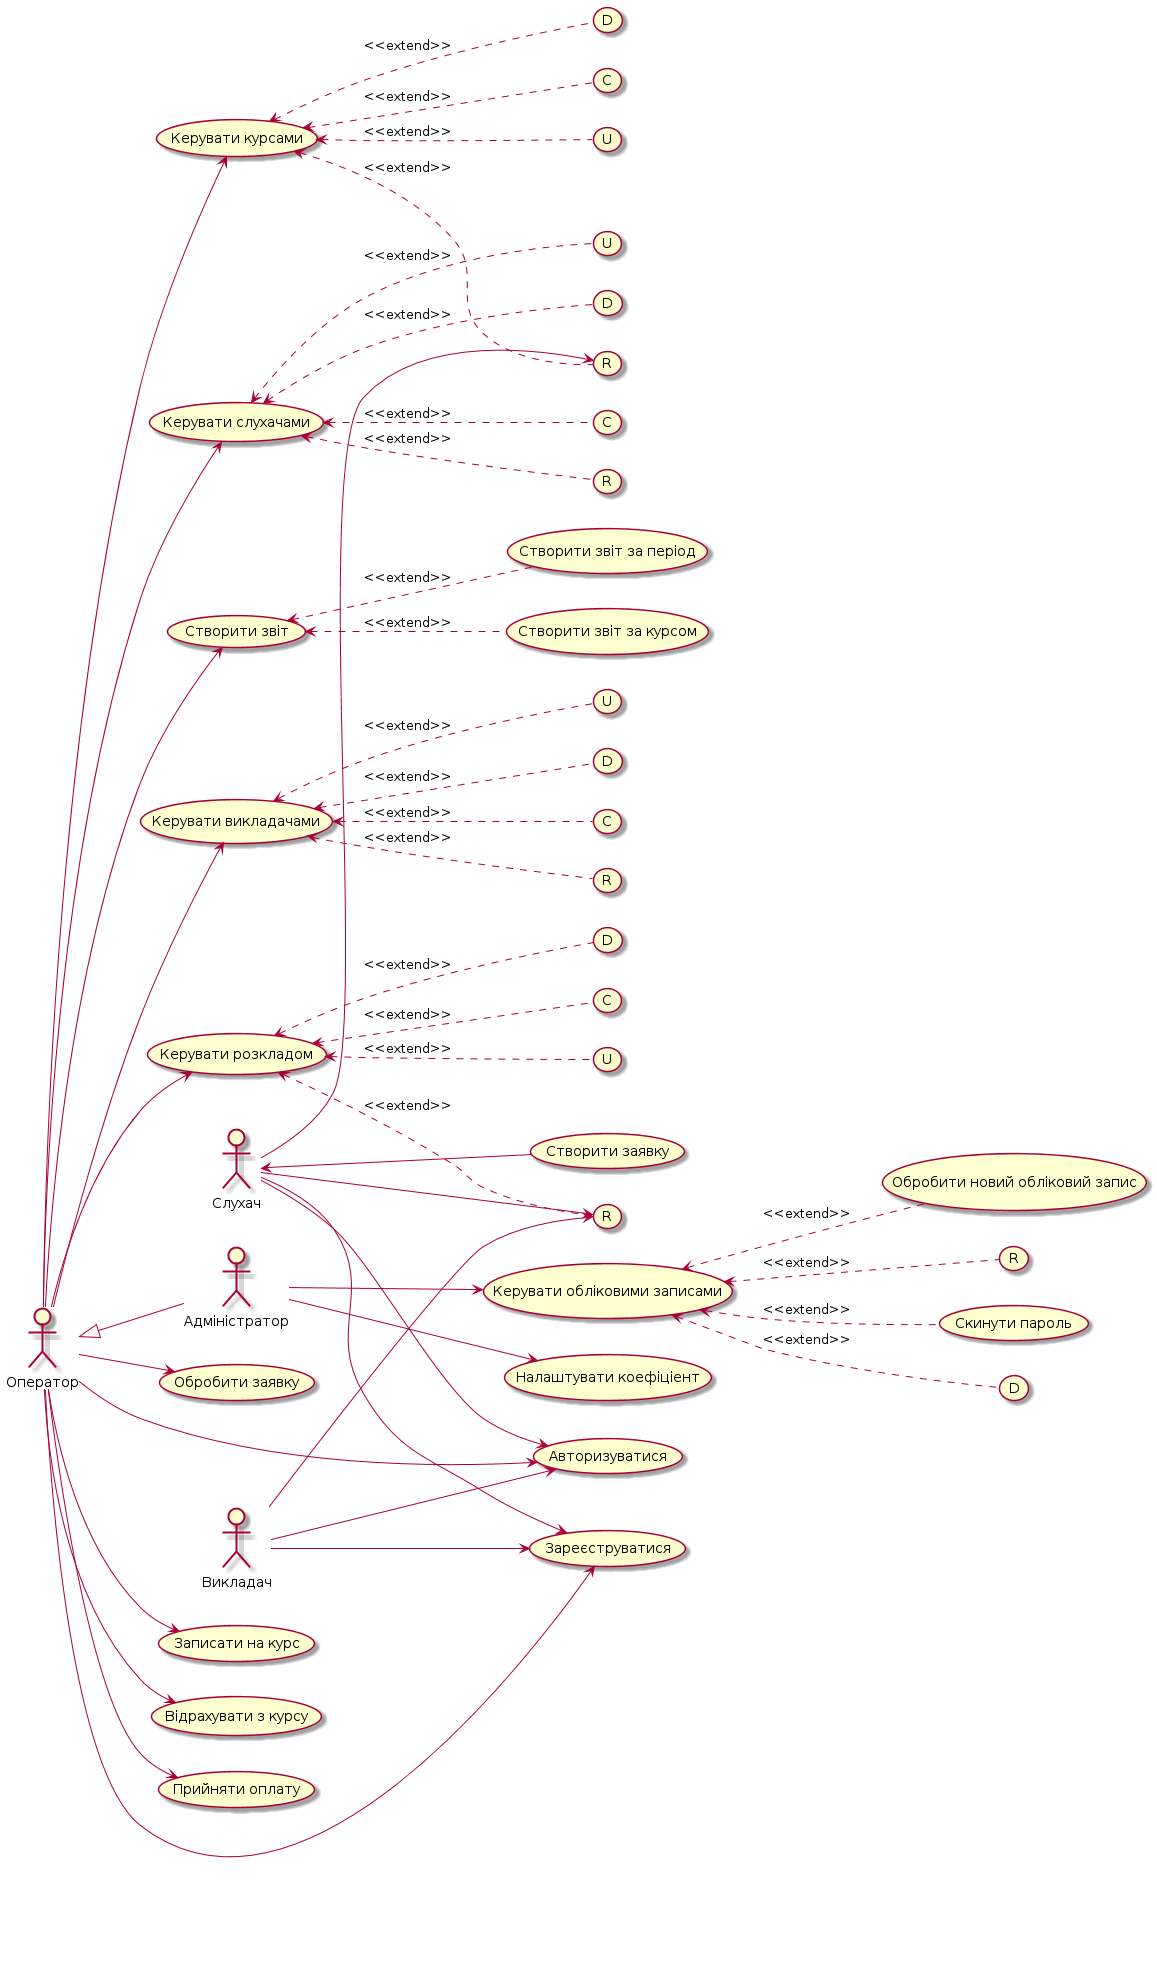
\includegraphics[width=12cm]{pp_pw1_uc.png}
\imglabel{Діаграма варіантів використання}

\newpage

\subsubsection{Опис варіантів використання}

\newcommand{\rowspan}[2]{
 \multirow{1}{*}[
  \dimexpr#1 / 2\relax
 ]{#2}
}

\newcounter{usecase_c}
\newcounter{scenario_c}
\newcounter{extension_c}
\newcounter{extensionset_c}
\newcounter{extension_for}
\newlength{\spanHeight}
\newbox\tmpparbox

\newcommand{\usecase}[9]{

 \stepcounter{usecase_c}
 \setcounter{scenario_c}{0}
 \setcounter{extension_c}{0}
 \setcounter{extension_for}{1}
 \setlength{\spanHeight}{0pt}

 \tablabel{#1}

 \nopagebreak[4]
 \begin{supertabular}{|p{4.6cm}|p{11.9cm}|}
 \hline Діючі особи & #2 \\
 \hline Область дії & #3 \\
 \hline Рівень & #4 \\
 \hline Учасники та інтереси & #5 \\
 \hline Передумови & #6 \\
 \hline Гарантії успіху & #7 \\
 \hline
 #8
 \hline
 #9
 \hline
 \end{supertabular}
 \\[5mm]
 \FloatBarrier
}
\def\auth{аутентифікований та авторизований}
\newcommand{\scenario}[1]{\stepcounter{scenario_c} &
 \global\sbox{\tmpparbox}{\parbox{11.9cm}{\arabic{scenario_c}. #1.}}
 \global\addtolength{\spanHeight}{\ht\tmpparbox}
 \global\addtolength{\spanHeight}{7pt}
 \arabic{scenario_c}. #1. \\ \cline{2-2}
}
\newcommand{\lastscenario}[1]{\stepcounter{scenario_c} \rowspan{\spanHeight}{Основний сценарій} \global\setlength{\spanHeight}{0pt} & \arabic{scenario_c}. #1. \\}
\newcommand{\extensionfor}[1]{\setcounter{extensionset_c}{0} \setcounter{extension_for}{\numexpr#1\relax}}
\newcommand{\extensionbox}[3]{
 #3 &
 \global\sbox{\tmpparbox}{\parbox{11.9cm}{\arabic{extension_for}.\Asbuk{extensionset_c}.#2 #1.}}
 \global\addtolength{\spanHeight}{\ht\tmpparbox}
 \global\addtolength{\spanHeight}{7pt}
 \arabic{extension_for}.\Asbuk{extensionset_c}.#2 #1.
}
\newcommand{\newextensionset}[1]{\stepcounter{extensionset_c} \setcounter{extension_c}{0} \extensionbox{#1}{}{} \\ \cline{2-2}}
\newcommand{\lastnewextensionset}[1]{\stepcounter{extensionset_c} \setcounter{extension_c}{0} \extensionbox{#1}{}{\rowspan{\spanHeight}{Розширення}} \\ \cline{2-2}}
\newcommand{\extension}[1]{\stepcounter{extension_c} \extensionbox{#1}{\arabic{extension_c}.}{} \\ \cline{2-2}}
\newcommand{\lastextension}[1]{\stepcounter{extension_c} \extensionbox{#1}{\arabic{extension_c}.}{\rowspan{\spanHeight}{Розширення}} \\}
\newcommand{\noext}{Розширення & ---\\}

\usecase{Видалити курс}{Оператор}{Система}{Мета користувача}{Оператор бажає прибрати з системи помилково створений або скасований курс}{Курс є в системі, оператор \auth}{Курс щез зі списку курсів}{
\scenario{Оператор обирає курс}
\lastscenario{Оператор видаляє обраний курс}
}{\noext}

\usecase{Додати курс}{Оператор}{Система}{Мета користувача}{Заплановано новий курс і оператор має намір відкрити на нього набір слухачів}{Курс відсутній в системі, оператор \auth}{Курс з'явився в системі}{
\scenario{Оператор створює новий курс}
\scenario{Оператор вводить інформацію про курс}
\lastscenario{Оператор зберігає курс}
}{
 \extensionfor{2}
 \newextensionset{Оператор не ввів назву курсу}
 \extension{Система вимагає ввести назву курсу}
 \lastextension{Перехід до п. 2}
}

\newpage
\usecase{Редагувати курс}{Оператор}{Система}{Мета користувача}{Змінилися характеристики існуючого курсу й оператор бажає оновити його дані в системі}{Курс є в системі, оператор \auth}{Система видає нові дані курсу}{
\scenario{Оператор обирає курс}
\scenario{Оператор змінює потрібні дані}
\lastscenario{Оператор зберігає курс}
}{\noext}

\usecase{Редагувати слухача}{Оператор}{Система}{Мета користувача}{Змінено чи уточнено ПІБ чи контактні дані слухача й оператор бажає оновити їх у системі}{Слухач є в системі, оператор \auth}{Система видає нові дані слухача}{
\scenario{Оператор обирає слухача}
\scenario{Оператор змінює потрібні дані}
\lastscenario{Оператор зберігає слухача}
}{\noext}

\newpage
\usecase{Видалити слухача}{Оператор}{Система}{Мета користувача}{Слухач так і не записався на жоден курс і тримати з ним зв'язок більше немає сенсу, тому оператор бажає видалити його з системи}{Слухач є в системі, оператор \auth}{Система не видає слухача}{
\scenario{Оператор обирає слухача}
\lastscenario{Оператор видаляє обраного слухача}
}{\noext}

\usecase{Переглянути курси}{Слухач, оператор}{Система}{Мета користувача}{Користувач бажає отримати перелік наявних у системі курсів для ознайомлення або, якщо це оператор --- для виконання операцій над ними}{Користувач \auth}{Користувач отримав перелік курсів}{
\lastscenario{Користувач запитує перегляд курсів}
}{\noext}

\newpage
\usecase{Додати слухача}{Оператор, слухач}{Система, кафедра СПЗ}{Мета користувача}{З'явився новий слухач, що не записувався через мережу Інтернет, і оператор бажає додати його до системи}{Слухач відсутній в системі, оператор \auth}{Слухач з'явився в системі}{
\scenario{Оператор створює нового слухача}
\scenario{Оператор запитує невідому йому інформацію у слухача}
\scenario{Оператор вводить інформацію про слухача}
\lastscenario{Оператор зберігає слухача}
}{\noext}

\usecase{Переглянути слухача}{Оператор}{Система}{Мета користувача}{Оператор бажає отримати перелік наявних у системі слухачів для ознайомлення чи виконання операцій над ними}{Оператор \auth}{Оператор отримав перелік слухачів}{
\lastscenario{Оператор запитує перегляд слухачів}
}{\noext}

\newpage
\usecase{Створити звіт за період}{Оператор}{Система}{Мета користувача}{Оператор бажає передати друкований звіт у бухгалтерію у кінці певного навчального періоду}{Оператор \auth}{Отримано придатний до друку документ, що містить звітність за курсами з заданого періоду}{
\scenario{Оператор обирає звіт за період}
\scenario{Оператор задає діапазон дат}
\lastscenario{Оператор підтверджує створення звіту}
}{
 \extensionfor{2}
 \newextensionset{Кінцева дата менше початкової або діапазон майбутній}
 \lastextension{Система повідомляє про невірний діапазон дат. Перехід до п.2}
}

\usecase{Створити звіт за курсом}{Оператор}{Система}{Мета користувача}{Оператор бажає передати друкований звіт у бухгалтерію по закінченню певного курсу}{Оператор \auth}{Отримано придатний до друку документ, що містить звітність за заданим курсом}{
\scenario{Оператор обирає курс}
\lastscenario{Оператор викликає створення звіту}
}{\noext}

\newpage
\usecase{Видалити розклад}{Оператор}{Система}{Мета користувача}{Курс перенесено на невизначений термін і поточний розклад для нього більше не актуальний, тож оператор бажає видалити цей розклад з системи}{Оператор \auth}{У курсу немає розкладу}{
\scenario{Оператор обирає курс}
\lastscenario{Оператор видаляє розклад для курсу}
}{\noext}

\usecase{Створити розклад}{Оператор}{Система}{Мета користувача}{Для нового курсу затверджено розклад і оператор бажає додати його до системи}{Оператор \auth}{На курс призначено введений розклад}{
\scenario{Оператор обирає курс}
\scenario{Оператор вводить дату проведення заняття та вказує тип заняття (лекція чи практика)}
\lastscenario{Оператор повторює п. 2 для всіх призначених занять}
}{
 \extensionfor{2}
 \newextensionset{Дата заняття виходить за діапазон дат проведення курсу}
 \lastextension{Система повідомляє про невірну дату. Перехід до п.2}
}

\newpage
\usecase{Редагування розкладу}{Оператор}{Система}{Мета користувача}{У розклад курсу внесено зміни й оператор бажає відбити їх у системі}{Оператор \auth}{На курс призначено відредагований розклад}{
\scenario{Оператор обирає курс}
\scenario{Оператор додає заняття, яких немає у збереженій версії розкладу}
\scenario{Оператор видаляє неактуальні заняття, які є у збереженій версії розкладу}
\scenario{Оператор змінює дату для занять, які перенесено}
\lastscenario{Оператор змінює тип для занять, які змінили тип порівняно зі збереженою версією розкладу}
}{
 \extensionfor{4}
 \newextensionset{Дата заняття виходить за діапазон дат проведення курсу}
 \lastextension{Система повідомляє про невірну дату. Перехід до п.4}
}

\usecase{Створити заявку}{Слухач, система}{Зовнішня система}{Мета користувача}{Слухач бажає зареєструватися на курс}{Оператор \auth\ у зовнішній системі}{Заявка з'явилася у сповіщення для операторів системи}{
\scenario{Слухач обирає курс}
\scenario{Слухач вводить свої ПІБ та контактні дані}
\lastscenario{Слухач відправляє заявку, зовнішня система передає заявку системі}
}{\noext}

\newpage
\usecase{Переглянути розклад}{Слухач, оператор, викладач}{Система, зовнішня система}{Мета користувача}{Користувач бажає переглянути розклад для певного курсу}{Оператор або викладач --- \auth\ у системі; слухач --- у зовнішній системі}{Користувач отримав розклад для обраного курсу}{
\scenario{Користувач обирає курс}
\lastscenario{Користувач запитує перегляд розкладу}
}{\noext}

\usecase{Обробити новий обліковий запис}{Адміністратор}{Система}{Мета користувача}{Адміністратор має намір обробити нові сповіщення}{Адміністратор \auth}{Обліковий запис доступний для аутентифікації або видалений}{
\scenario{Адміністратор обирає сповіщення}
\lastscenario{Адміністратор підтверджує сповіщення}
}{
 \extensionfor{2}
 \lastnewextensionset{Адміністратор відхилює сповіщення}
}

\usecase{Переглянути облікові записи}{Адміністратор}{Система}{Мета користувача}{Адміністратор бажає ознайомитися з тим, які користувачі наразі є в системі та які вони мають рівні прав доступу}{Адміністратор \auth}{Адміністратор отримав перелік облікових записів}{
\lastscenario{Адміністратор запитує перегляд облікових записів}
}{\noext}

\newpage
\usecase{Скинути пароль}{Адміністратор, користувач}{Система}{Мета користувача}{До адміністратора особисто звернувся користувач, який забув пароль, і адміністратор згоден скинути пароль, щоб користувач встановив новий}{Адміністратор \auth}{Користувач може повторно аутентифікуватися з новим паролем}{
\scenario{Адміністратор обирає обліковий запис користувача}
\scenario{Адміністратор викликає скидання паролю}
\lastscenario{Користувач заходить в систему зі своїм логіном та новим паролем}
}{\noext}

\usecase{Видалити обліковий запис}{Адміністратор}{Система}{Мета користувача}{Адміністратор бажає видалити обліковий запис користувача, якому більше не потрібен доступ до системи у якості оператора, адміністратора чи викладача}{Адміністратор \auth}{Обраний обліковий запис більше недоступний для аутентифікації та відсутній у переліку облікових записів}{
\scenario{Адміністратор обирає обліковий запис}
\lastscenario{Адміністратор видаляє обраний обліковий запис}
}{\noext}

\newpage
\usecase{Налаштувати коефіціент}{Адміністратор}{Система}{Мета користувача}{Змінилися коефіціенти розрахунку вартості курсу і адміністратор бажає відкорегувати автоматичний розрахунок}{Адміністратор \auth}{Вартості курсу розраховуються з урахуванням нового коефіціенту}{
\scenario{Адміністратор обирає коефіціент}
\lastscenario{Адміністратор встановлює нове значення коефіціенту}
}{\noext}

\usecase{Обробити заявку}{Оператор, слухач}{Система}{Мета користувача}{Оператор має намір обробити нові сповіщення}{Оператор \auth}{Слухач із вказаними в заявці даними з'явився в системі та записаний на вказаний у заявці курс або заявка просто зникла зі сповіщень}{
\scenario{Оператор обирає сповіщення}
\scenario{Оператор підтверджує додання даних з заявки}
\scenario{Система впевнюється, що слухача, який подав в заявку, ще не додано до системи}
\scenario{Система формує форму заповнену форму договору для друку}
\lastscenario{Оператор роздруковує форму, слухач приходить на кафедру СПЗ і підписує}
}{
 \extensionfor{2}
 \newextensionset{Оператор відхиляє додання даних з заявки}
 \extensionfor{3}
 \newextensionset{Слухач, що подаяв заявку, вже існує в системі}
 \extension{Оператор обирає слухача}
 \lastextension{Оператор зливає дані користувача з даними заявки. Перехід до п. 4}
}

\usecase{Авторизуватися}{Користувач}{Система}{Мета користувача}{Користувач має намір проводити певні дії у системі}{Користувач має обліковий запис у системі}{Користувач авторизований}{
\lastscenario{Користувач вводить логін та пароль}
}{
 \extensionfor{1}
 \newextensionset{Користувач із таким логіном не існує або пароль невірний}
 \lastscenario{Система повідомляє про відхилення авторизації. Перехід до п.1}
}

\usecase{Зареєструватися}{Користувач}{Система}{Мета користувача}{Користувач має намір проводити певні дії у системі}{Користувач не має облікового запису у системі}{Адміністратори отримали сповіщення про реєстрацію нового користувача, обліковий запис не доступний для аутентифікації}{
\lastscenario{Користувач вводить логін та пароль}
}{
 \extensionfor{1}
 \newextensionset{Користувач із таким логіном вже існує}
 \lastextension{Система повідомляє слухачеві, що слід обрати інший логін. Перехід до п.1}
}

\newpage
\usecase{Записати слухача на курс}{Оператор, слухач}{Система}{Мета користувача}{Слухач сповістив, що бажає записатися на курс, але не подавав заявку через мережу Інтернет, і оператор бажає самостійно записати його на курс}{Слухач присутній у системі, оператор \auth}{Слухач є серед слухачів курсу}{
\scenario{Оператор обирає слухача}
\scenario{Оператор обирає курс}
\scenario{Оператор записує слухача на курс}
\scenario{Система формує заповнену форму договору для друку}
\lastscenario{Оператор роздруковує форму, слухач підписує}
}{\noext}

\usecase{Відрахувати слухача з курсу}{Оператор}{Система}{Мета користувача}{Слухач передумав або не сплатив вчасно курс і не відвідує заняття}{Слухач присутній у системі і записаний на курс, оператор \auth}{Слухача немає серед слухачів курсу}{
\scenario{Оператор обирає слухача}
\scenario{Оператор обирає курс}
\scenario{Оператор запитує сплачену слухачем суму. Система відповідає}
\scenario{Оператор повертає слухачеві сплачені кошти}
\lastscenario{Оператор відраховує слухача з курсу}
}{
 \extensionfor{3}
 \newextensionset{Слухач не сплачував кошти за курс}
 \lastextension{Перехід до п.5}
}

\newpage
\usecase{Прийняти оплату}{Оператор, слухач}{Система, кафедра СПЗ}{Мета користувача}{Слухач приніс певну суму коштів і оператор бажає внести її до системи}{Слухач присутній у системі і записаний на курс, оператор \auth}{Загальна оплата слухачем за курс змінилася на прийняту суму}{
\scenario{Оператор приймає та перераховує кошти}
\scenario{Оператор обирає слухача}
\scenario{Оператор обирає курс}
\scenario{Оператор впевнюється, що слухач має заборгованість за курс}
\lastscenario{Оператор вводить суму коштів}
}{
 \extensionfor{4}
 \newextensionset{Слухач приніс більше коштів, ніж має заборгованість}
 \extension{Оператор вводить суму, рівну боргу слухача}
 \extension{Оператор повертає слухачеві здачу}
 \newextensionset{Слухач не має заборгованості}
 \lastextension{Оператор повертає слухачеві кошти}
}
